\subsection{Preambulo}
El objetivo de este trabajo practico será la implementacion y la experimentacion sobre diversos tipos de schedulers. El proposito de esto será ver cuales son sus ventajas, cuales sus desventajas y cual es más conveniente para determinado set de tareas.
\\
Para ello contaremos con un simulador que actuará como un sistema operativo y que entregará tareas para que cada scheduler corra. Estas tareas serán definidas de antemano, pudiendo simular en ellas un uso intensivo del CPU o una llamada bloqueante del sistema que equivaldrá a que la tarea deba esperar algun recurso del sistema.
\\
Para este trabajo implementaremos un scheduler Round Robin simple, un Round Robin que no permita la migración de procesos entre nucleos, más otros dos schedulers descriptos en el paper de C. L. Liu. Además la cátedra nos provee de un scheduler First Come First Served que utilizaremos para comparar los otros schedulers y sacar conclusiones de los mismos.
\subsection{Metricas a utilizar}

Para medir que tan 'buenos' son los algoritmos utilizados, empelaremos dos metricas distintas: Turnaround y Waiting Time.
\\
Turnaround hará referencia a cuanto tarda un proceso en terminar de ejecutarse desde la primera vez que esta en ready. Esta metrica será buena para medir procesos que utilicen muchos recursos de la CPU ya que esta fuertemente ligado a cuanto quantum esta asignandole el procesador a ese proceso en particular.
\\
La segunda metrica sera Waiting time, y será util para medir tareas que permanezcan mucho tiempo bloqueadas, ya sea por llamadas al sistema, esperen algun input en especial, etc. Es claro que estas tareas no dependen de su tiempo de ejecucion sino de que sean atendidas lo mas rapidamete posibles, O por decirlo de otra manera, se buscará minimizar el tiempo entre que una tarea deja de estar bloqueada y su nueva ejecución.
\\
El lector puede notar que estas dos metricas son bastante contradictorias ya que, para minimizar el turnaround uno tenderia a asignarle la mayor cantidad de recursos posibles a una tarea especifica. Pero esto probocara que las demas tareas no sean atendidas y permanezcan mucho tiempo a la espera. Por otra parte para intentar mejorar el waiting time uno podria elegir un quantum pequeño para cada una de las tareas y que se rote entre ellas de manera constante. Esto sin duda probocará que el procesador este realizando constantes context switches y probocara un peor tiempo en el turnarround.
\\
A manera de introducción, en la siguiente sección se implementarán algunas tareas simples las cuales correremos sobre el scheduler provisto por la catedra para intentar sacar alguas conclusiones preliminares.
\subsection{Experimentacion Preliminar Sobre Scheduler FCFS}

Para esta experimentación primero implementaremos una tarea a la que denominaremos TaskConsola, que simulará una tarea interactiva. La misma contara con $n$ llamadas bloqueantes al sistema de un tiempo aleatorio pasado por parámetro.
\\
Luego crearemos un lote de tareas a ejecutar por el simulador, una que utilice de manera intensiva el CPU, y dos TaskConsola.
\\
Lo obtenido puede verse en el siguiente grafico:
\\
\begin{figure}[H]
  \centering
	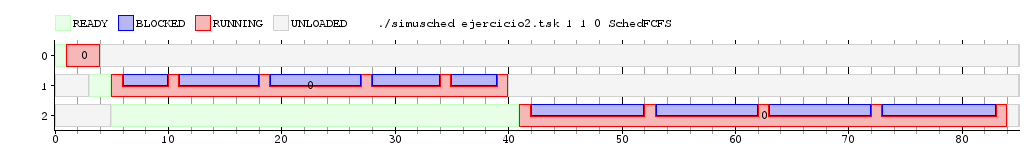
\includegraphics[scale=0.45]{graficos/parte1/testFCFS.png}
  \caption[Caption for LOF]{}
\end{figure}
A simple vista puede verse cual es uno de los problemas fundamentales con este scheduler. Cuando la tarea 1 esta bloqueada en espera de algun recurso, el procesador, en vez de cambiar de tarea y intentar adelantar alguna otra, no esta siendo utilizado para nada lo que es sin duda una desventaja tanto para el turnaround, ya que otras tareas podrian terminar antes si se ejecutaran, como para el waiting time, ya que se ve claramente que la tarea 2 esta teniendo que esperar un gran tiempo sin ser ejecutada.
\\
Ademas, si se diera el caso en que un gran numero de tareas esten esperando para ser ejecutadas, y la primera tarea, por la razon que sea, nunca termine, entonces todas las demas tareas sufrirán de inanición.
\\
Aun así este tipo de shceduler puede ser util, ya que es muy facil de implementar y es posible hacerlo en sistemas donde no se cuentan con interrupciones temporales de las que el kernel pueda hacer uso.
\\
En los siguientes apartados pasaremos a describir e implementar varios schedulers de mayor complegidad que intenten lidiar con los problemas descriptos anteriormente, esto es, schedulers que permitan aprovechar los tiempos muertos en los que la tarea en ejecucion debe esperar por algun recurso y que tenga sierto grado de 'justicia' para que ninguna tarea sufra de inanición. Ademas realizaremos diversas experimentaciones para ver que ventajas y desventajas con la utilizacion de cada uno.
